
\begin{figure}[H]

  \centering

  \begin{tikzpicture}
    \fill[gray] (0, 0) rectangle (1, 1);
    \fill[gray] (2, 0) rectangle (3, 1);
    \fill[gray] (4, 0) rectangle (5, 1);
    \fill[gray] (0, 1) rectangle (1, 2);
    \fill[gray] (2, 1) rectangle (3, 2);
    \node at (0.5, 2.5){\color{blue}\faIcon{user}};
    \fill[gray] (4, 2) rectangle (5, 3);
    \fill[gray] (2, 3) rectangle (3, 4);
    \fill[gray] (4, 3) rectangle (5, 4);
    \fill[gray] (0, 4) rectangle (1, 5);
    \fill[gray] (2, 4) rectangle (3, 5);
    \node at (3.5, 4.5){\color{blue}\faIcon{home}};
    \fill[gray] (4, 4) rectangle (5, 5);
    \draw[black] grid (5, 5);
  \end{tikzpicture}

  \caption{Dodaj do kolejki węzeł x: 0 y: 2}
  \label{fig:bfs_solve_steps}
\end{figure}

\begin{figure}[H]
  \ContinuedFloat
  \centering

  \begin{tikzpicture}
    \fill[gray] (0, 0) rectangle (1, 1);
    \fill[gray] (2, 0) rectangle (3, 1);
    \fill[gray] (4, 0) rectangle (5, 1);
    \fill[gray] (0, 1) rectangle (1, 2);
    \fill[gray] (2, 1) rectangle (3, 2);
    \node at (0.5, 2.5){\color{blue}\faIcon{user}};
    \fill[gray] (4, 2) rectangle (5, 3);
    \fill[gray] (2, 3) rectangle (3, 4);
    \fill[gray] (4, 3) rectangle (5, 4);
    \fill[gray] (0, 4) rectangle (1, 5);
    \fill[gray] (2, 4) rectangle (3, 5);
    \node at (3.5, 4.5){\color{blue}\faIcon{home}};
    \fill[gray] (4, 4) rectangle (5, 5);
    \draw[black] grid (5, 5);
  \end{tikzpicture}

  \caption{Rozpatrz x: 0 y: 2}

\end{figure}

\begin{figure}[H]
  \ContinuedFloat
  \centering

  \begin{tikzpicture}
    \fill[gray] (0, 0) rectangle (1, 1);
    \fill[gray] (2, 0) rectangle (3, 1);
    \fill[gray] (4, 0) rectangle (5, 1);
    \fill[gray] (0, 1) rectangle (1, 2);
    \fill[gray] (2, 1) rectangle (3, 2);
    \node at (0.5, 2.5){\color{blue}\faIcon{user}};
    \node at (1.5, 2.5){\color{purple}\faIcon{hourglass}};
    \fill[gray] (4, 2) rectangle (5, 3);
    \fill[gray] (2, 3) rectangle (3, 4);
    \fill[gray] (4, 3) rectangle (5, 4);
    \fill[gray] (0, 4) rectangle (1, 5);
    \fill[gray] (2, 4) rectangle (3, 5);
    \node at (3.5, 4.5){\color{blue}\faIcon{home}};
    \fill[gray] (4, 4) rectangle (5, 5);
    \draw[black] grid (5, 5);
  \end{tikzpicture}

  \caption{Dodaj do kolejki węzeł x: 1 y: 2}

\end{figure}

\begin{figure}[H]
  \ContinuedFloat
  \centering

  \begin{tikzpicture}
    \fill[gray] (0, 0) rectangle (1, 1);
    \fill[gray] (2, 0) rectangle (3, 1);
    \fill[gray] (4, 0) rectangle (5, 1);
    \fill[gray] (0, 1) rectangle (1, 2);
    \fill[gray] (2, 1) rectangle (3, 2);
    \node at (0.5, 2.5){\color{blue}\faIcon{user}};
    \node at (1.5, 2.5){\color{purple}\faIcon{hourglass}};
    \fill[gray] (4, 2) rectangle (5, 3);
    \node at (0.5, 3.5){\color{purple}\faIcon{hourglass}};
    \fill[gray] (2, 3) rectangle (3, 4);
    \fill[gray] (4, 3) rectangle (5, 4);
    \fill[gray] (0, 4) rectangle (1, 5);
    \fill[gray] (2, 4) rectangle (3, 5);
    \node at (3.5, 4.5){\color{blue}\faIcon{home}};
    \fill[gray] (4, 4) rectangle (5, 5);
    \draw[black] grid (5, 5);
  \end{tikzpicture}

  \caption{Dodaj do kolejki węzeł x: 0 y: 3}

\end{figure}

\begin{figure}[H]
  \ContinuedFloat
  \centering

  \begin{tikzpicture}
    \fill[gray] (0, 0) rectangle (1, 1);
    \fill[gray] (2, 0) rectangle (3, 1);
    \fill[gray] (4, 0) rectangle (5, 1);
    \fill[gray] (0, 1) rectangle (1, 2);
    \fill[gray] (2, 1) rectangle (3, 2);
    \node at (0.5, 2.5){\color{blue}\faIcon{user}};
    \node at (1.5, 2.5){\color{orange}\faIcon{arrows-alt}};
    \fill[gray] (4, 2) rectangle (5, 3);
    \node at (0.5, 3.5){\color{purple}\faIcon{hourglass}};
    \fill[gray] (2, 3) rectangle (3, 4);
    \fill[gray] (4, 3) rectangle (5, 4);
    \fill[gray] (0, 4) rectangle (1, 5);
    \fill[gray] (2, 4) rectangle (3, 5);
    \node at (3.5, 4.5){\color{blue}\faIcon{home}};
    \fill[gray] (4, 4) rectangle (5, 5);
    \draw[black] grid (5, 5);
  \end{tikzpicture}

  \caption{Rozpatrz x: 1 y: 2}

\end{figure}

\begin{figure}[H]
  \ContinuedFloat
  \centering

  \begin{tikzpicture}
    \fill[gray] (0, 0) rectangle (1, 1);
    \fill[gray] (2, 0) rectangle (3, 1);
    \fill[gray] (4, 0) rectangle (5, 1);
    \fill[gray] (0, 1) rectangle (1, 2);
    \fill[gray] (2, 1) rectangle (3, 2);
    \node at (0.5, 2.5){\color{blue}\faIcon{user}};
    \node at (1.5, 2.5){\color{orange}\faIcon{arrows-alt}};
    \fill[gray] (4, 2) rectangle (5, 3);
    \node at (0.5, 3.5){\color{purple}\faIcon{hourglass}};
    \fill[gray] (2, 3) rectangle (3, 4);
    \fill[gray] (4, 3) rectangle (5, 4);
    \fill[gray] (0, 4) rectangle (1, 5);
    \fill[gray] (2, 4) rectangle (3, 5);
    \node at (3.5, 4.5){\color{blue}\faIcon{home}};
    \fill[gray] (4, 4) rectangle (5, 5);
    \draw[black] grid (5, 5);
  \end{tikzpicture}

  \caption{Dodaj do kolejki węzeł x: 0 y: 2}

\end{figure}

\begin{figure}[H]
  \ContinuedFloat
  \centering

  \begin{tikzpicture}
    \fill[gray] (0, 0) rectangle (1, 1);
    \fill[gray] (2, 0) rectangle (3, 1);
    \fill[gray] (4, 0) rectangle (5, 1);
    \fill[gray] (0, 1) rectangle (1, 2);
    \node at (1.5, 1.5){\color{purple}\faIcon{hourglass}};
    \fill[gray] (2, 1) rectangle (3, 2);
    \node at (0.5, 2.5){\color{blue}\faIcon{user}};
    \node at (1.5, 2.5){\color{orange}\faIcon{arrows-alt}};
    \fill[gray] (4, 2) rectangle (5, 3);
    \node at (0.5, 3.5){\color{purple}\faIcon{hourglass}};
    \fill[gray] (2, 3) rectangle (3, 4);
    \fill[gray] (4, 3) rectangle (5, 4);
    \fill[gray] (0, 4) rectangle (1, 5);
    \fill[gray] (2, 4) rectangle (3, 5);
    \node at (3.5, 4.5){\color{blue}\faIcon{home}};
    \fill[gray] (4, 4) rectangle (5, 5);
    \draw[black] grid (5, 5);
  \end{tikzpicture}

  \caption{Dodaj do kolejki węzeł x: 1 y: 1}

\end{figure}

\begin{figure}[H]
  \ContinuedFloat
  \centering

  \begin{tikzpicture}
    \fill[gray] (0, 0) rectangle (1, 1);
    \fill[gray] (2, 0) rectangle (3, 1);
    \fill[gray] (4, 0) rectangle (5, 1);
    \fill[gray] (0, 1) rectangle (1, 2);
    \node at (1.5, 1.5){\color{purple}\faIcon{hourglass}};
    \fill[gray] (2, 1) rectangle (3, 2);
    \node at (0.5, 2.5){\color{blue}\faIcon{user}};
    \node at (1.5, 2.5){\color{orange}\faIcon{arrows-alt}};
    \fill[gray] (4, 2) rectangle (5, 3);
    \node at (0.5, 3.5){\color{purple}\faIcon{hourglass}};
    \node at (1.5, 3.5){\color{purple}\faIcon{hourglass}};
    \fill[gray] (2, 3) rectangle (3, 4);
    \fill[gray] (4, 3) rectangle (5, 4);
    \fill[gray] (0, 4) rectangle (1, 5);
    \fill[gray] (2, 4) rectangle (3, 5);
    \node at (3.5, 4.5){\color{blue}\faIcon{home}};
    \fill[gray] (4, 4) rectangle (5, 5);
    \draw[black] grid (5, 5);
  \end{tikzpicture}

  \caption{Dodaj do kolejki węzeł x: 1 y: 3}

\end{figure}

\begin{figure}[H]
  \ContinuedFloat
  \centering

  \begin{tikzpicture}
    \fill[gray] (0, 0) rectangle (1, 1);
    \fill[gray] (2, 0) rectangle (3, 1);
    \fill[gray] (4, 0) rectangle (5, 1);
    \fill[gray] (0, 1) rectangle (1, 2);
    \node at (1.5, 1.5){\color{purple}\faIcon{hourglass}};
    \fill[gray] (2, 1) rectangle (3, 2);
    \node at (0.5, 2.5){\color{blue}\faIcon{user}};
    \node at (1.5, 2.5){\color{orange}\faIcon{arrows-alt}};
    \node at (2.5, 2.5){\color{purple}\faIcon{hourglass}};
    \fill[gray] (4, 2) rectangle (5, 3);
    \node at (0.5, 3.5){\color{purple}\faIcon{hourglass}};
    \node at (1.5, 3.5){\color{purple}\faIcon{hourglass}};
    \fill[gray] (2, 3) rectangle (3, 4);
    \fill[gray] (4, 3) rectangle (5, 4);
    \fill[gray] (0, 4) rectangle (1, 5);
    \fill[gray] (2, 4) rectangle (3, 5);
    \node at (3.5, 4.5){\color{blue}\faIcon{home}};
    \fill[gray] (4, 4) rectangle (5, 5);
    \draw[black] grid (5, 5);
  \end{tikzpicture}

  \caption{Dodaj do kolejki węzeł x: 2 y: 2}

\end{figure}

\begin{figure}[H]
  \ContinuedFloat
  \centering

  \begin{tikzpicture}
    \fill[gray] (0, 0) rectangle (1, 1);
    \fill[gray] (2, 0) rectangle (3, 1);
    \fill[gray] (4, 0) rectangle (5, 1);
    \fill[gray] (0, 1) rectangle (1, 2);
    \node at (1.5, 1.5){\color{purple}\faIcon{hourglass}};
    \fill[gray] (2, 1) rectangle (3, 2);
    \node at (0.5, 2.5){\color{blue}\faIcon{user}};
    \node at (1.5, 2.5){\color{orange}\faIcon{arrows-alt}};
    \node at (2.5, 2.5){\color{purple}\faIcon{hourglass}};
    \fill[gray] (4, 2) rectangle (5, 3);
    \node at (0.5, 3.5){\color{orange}\faIcon{arrows-alt}};
    \node at (1.5, 3.5){\color{purple}\faIcon{hourglass}};
    \fill[gray] (2, 3) rectangle (3, 4);
    \fill[gray] (4, 3) rectangle (5, 4);
    \fill[gray] (0, 4) rectangle (1, 5);
    \fill[gray] (2, 4) rectangle (3, 5);
    \node at (3.5, 4.5){\color{blue}\faIcon{home}};
    \fill[gray] (4, 4) rectangle (5, 5);
    \draw[black] grid (5, 5);
  \end{tikzpicture}

  \caption{Rozpatrz x: 0 y: 3}

\end{figure}

\begin{figure}[H]
  \ContinuedFloat
  \centering

  \begin{tikzpicture}
    \fill[gray] (0, 0) rectangle (1, 1);
    \fill[gray] (2, 0) rectangle (3, 1);
    \fill[gray] (4, 0) rectangle (5, 1);
    \fill[gray] (0, 1) rectangle (1, 2);
    \node at (1.5, 1.5){\color{purple}\faIcon{hourglass}};
    \fill[gray] (2, 1) rectangle (3, 2);
    \node at (0.5, 2.5){\color{blue}\faIcon{user}};
    \node at (1.5, 2.5){\color{orange}\faIcon{arrows-alt}};
    \node at (2.5, 2.5){\color{purple}\faIcon{hourglass}};
    \fill[gray] (4, 2) rectangle (5, 3);
    \node at (0.5, 3.5){\color{orange}\faIcon{arrows-alt}};
    \node at (1.5, 3.5){\color{purple}\faIcon{hourglass}};
    \fill[gray] (2, 3) rectangle (3, 4);
    \fill[gray] (4, 3) rectangle (5, 4);
    \fill[gray] (0, 4) rectangle (1, 5);
    \fill[gray] (2, 4) rectangle (3, 5);
    \node at (3.5, 4.5){\color{blue}\faIcon{home}};
    \fill[gray] (4, 4) rectangle (5, 5);
    \draw[black] grid (5, 5);
  \end{tikzpicture}

  \caption{Rozpatrz x: 0 y: 2}

\end{figure}

\begin{figure}[H]
  \ContinuedFloat
  \centering

  \begin{tikzpicture}
    \fill[gray] (0, 0) rectangle (1, 1);
    \fill[gray] (2, 0) rectangle (3, 1);
    \fill[gray] (4, 0) rectangle (5, 1);
    \fill[gray] (0, 1) rectangle (1, 2);
    \node at (1.5, 1.5){\color{orange}\faIcon{arrows-alt}};
    \fill[gray] (2, 1) rectangle (3, 2);
    \node at (0.5, 2.5){\color{blue}\faIcon{user}};
    \node at (1.5, 2.5){\color{orange}\faIcon{arrows-alt}};
    \node at (2.5, 2.5){\color{purple}\faIcon{hourglass}};
    \fill[gray] (4, 2) rectangle (5, 3);
    \node at (0.5, 3.5){\color{orange}\faIcon{arrows-alt}};
    \node at (1.5, 3.5){\color{purple}\faIcon{hourglass}};
    \fill[gray] (2, 3) rectangle (3, 4);
    \fill[gray] (4, 3) rectangle (5, 4);
    \fill[gray] (0, 4) rectangle (1, 5);
    \fill[gray] (2, 4) rectangle (3, 5);
    \node at (3.5, 4.5){\color{blue}\faIcon{home}};
    \fill[gray] (4, 4) rectangle (5, 5);
    \draw[black] grid (5, 5);
  \end{tikzpicture}

  \caption{Rozpatrz x: 1 y: 1}

\end{figure}

\begin{figure}[H]
  \ContinuedFloat
  \centering

  \begin{tikzpicture}
    \fill[gray] (0, 0) rectangle (1, 1);
    \node at (1.5, 0.5){\color{purple}\faIcon{hourglass}};
    \fill[gray] (2, 0) rectangle (3, 1);
    \fill[gray] (4, 0) rectangle (5, 1);
    \fill[gray] (0, 1) rectangle (1, 2);
    \node at (1.5, 1.5){\color{orange}\faIcon{arrows-alt}};
    \fill[gray] (2, 1) rectangle (3, 2);
    \node at (0.5, 2.5){\color{blue}\faIcon{user}};
    \node at (1.5, 2.5){\color{orange}\faIcon{arrows-alt}};
    \node at (2.5, 2.5){\color{purple}\faIcon{hourglass}};
    \fill[gray] (4, 2) rectangle (5, 3);
    \node at (0.5, 3.5){\color{orange}\faIcon{arrows-alt}};
    \node at (1.5, 3.5){\color{purple}\faIcon{hourglass}};
    \fill[gray] (2, 3) rectangle (3, 4);
    \fill[gray] (4, 3) rectangle (5, 4);
    \fill[gray] (0, 4) rectangle (1, 5);
    \fill[gray] (2, 4) rectangle (3, 5);
    \node at (3.5, 4.5){\color{blue}\faIcon{home}};
    \fill[gray] (4, 4) rectangle (5, 5);
    \draw[black] grid (5, 5);
  \end{tikzpicture}

  \caption{Dodaj do kolejki węzeł x: 1 y: 0}

\end{figure}

\begin{figure}[H]
  \ContinuedFloat
  \centering

  \begin{tikzpicture}
    \fill[gray] (0, 0) rectangle (1, 1);
    \node at (1.5, 0.5){\color{purple}\faIcon{hourglass}};
    \fill[gray] (2, 0) rectangle (3, 1);
    \fill[gray] (4, 0) rectangle (5, 1);
    \fill[gray] (0, 1) rectangle (1, 2);
    \node at (1.5, 1.5){\color{orange}\faIcon{arrows-alt}};
    \fill[gray] (2, 1) rectangle (3, 2);
    \node at (0.5, 2.5){\color{blue}\faIcon{user}};
    \node at (1.5, 2.5){\color{orange}\faIcon{arrows-alt}};
    \node at (2.5, 2.5){\color{purple}\faIcon{hourglass}};
    \fill[gray] (4, 2) rectangle (5, 3);
    \node at (0.5, 3.5){\color{orange}\faIcon{arrows-alt}};
    \node at (1.5, 3.5){\color{orange}\faIcon{arrows-alt}};
    \fill[gray] (2, 3) rectangle (3, 4);
    \fill[gray] (4, 3) rectangle (5, 4);
    \fill[gray] (0, 4) rectangle (1, 5);
    \fill[gray] (2, 4) rectangle (3, 5);
    \node at (3.5, 4.5){\color{blue}\faIcon{home}};
    \fill[gray] (4, 4) rectangle (5, 5);
    \draw[black] grid (5, 5);
  \end{tikzpicture}

  \caption{Rozpatrz x: 1 y: 3}

\end{figure}

\begin{figure}[H]
  \ContinuedFloat
  \centering

  \begin{tikzpicture}
    \fill[gray] (0, 0) rectangle (1, 1);
    \node at (1.5, 0.5){\color{purple}\faIcon{hourglass}};
    \fill[gray] (2, 0) rectangle (3, 1);
    \fill[gray] (4, 0) rectangle (5, 1);
    \fill[gray] (0, 1) rectangle (1, 2);
    \node at (1.5, 1.5){\color{orange}\faIcon{arrows-alt}};
    \fill[gray] (2, 1) rectangle (3, 2);
    \node at (0.5, 2.5){\color{blue}\faIcon{user}};
    \node at (1.5, 2.5){\color{orange}\faIcon{arrows-alt}};
    \node at (2.5, 2.5){\color{purple}\faIcon{hourglass}};
    \fill[gray] (4, 2) rectangle (5, 3);
    \node at (0.5, 3.5){\color{orange}\faIcon{arrows-alt}};
    \node at (1.5, 3.5){\color{orange}\faIcon{arrows-alt}};
    \fill[gray] (2, 3) rectangle (3, 4);
    \fill[gray] (4, 3) rectangle (5, 4);
    \fill[gray] (0, 4) rectangle (1, 5);
    \node at (1.5, 4.5){\color{purple}\faIcon{hourglass}};
    \fill[gray] (2, 4) rectangle (3, 5);
    \node at (3.5, 4.5){\color{blue}\faIcon{home}};
    \fill[gray] (4, 4) rectangle (5, 5);
    \draw[black] grid (5, 5);
  \end{tikzpicture}

  \caption{Dodaj do kolejki węzeł x: 1 y: 4}

\end{figure}

\begin{figure}[H]
  \ContinuedFloat
  \centering

  \begin{tikzpicture}
    \fill[gray] (0, 0) rectangle (1, 1);
    \node at (1.5, 0.5){\color{purple}\faIcon{hourglass}};
    \fill[gray] (2, 0) rectangle (3, 1);
    \fill[gray] (4, 0) rectangle (5, 1);
    \fill[gray] (0, 1) rectangle (1, 2);
    \node at (1.5, 1.5){\color{orange}\faIcon{arrows-alt}};
    \fill[gray] (2, 1) rectangle (3, 2);
    \node at (0.5, 2.5){\color{blue}\faIcon{user}};
    \node at (1.5, 2.5){\color{orange}\faIcon{arrows-alt}};
    \node at (2.5, 2.5){\color{orange}\faIcon{arrows-alt}};
    \fill[gray] (4, 2) rectangle (5, 3);
    \node at (0.5, 3.5){\color{orange}\faIcon{arrows-alt}};
    \node at (1.5, 3.5){\color{orange}\faIcon{arrows-alt}};
    \fill[gray] (2, 3) rectangle (3, 4);
    \fill[gray] (4, 3) rectangle (5, 4);
    \fill[gray] (0, 4) rectangle (1, 5);
    \node at (1.5, 4.5){\color{purple}\faIcon{hourglass}};
    \fill[gray] (2, 4) rectangle (3, 5);
    \node at (3.5, 4.5){\color{blue}\faIcon{home}};
    \fill[gray] (4, 4) rectangle (5, 5);
    \draw[black] grid (5, 5);
  \end{tikzpicture}

  \caption{Rozpatrz x: 2 y: 2}

\end{figure}

\begin{figure}[H]
  \ContinuedFloat
  \centering

  \begin{tikzpicture}
    \fill[gray] (0, 0) rectangle (1, 1);
    \node at (1.5, 0.5){\color{purple}\faIcon{hourglass}};
    \fill[gray] (2, 0) rectangle (3, 1);
    \fill[gray] (4, 0) rectangle (5, 1);
    \fill[gray] (0, 1) rectangle (1, 2);
    \node at (1.5, 1.5){\color{orange}\faIcon{arrows-alt}};
    \fill[gray] (2, 1) rectangle (3, 2);
    \node at (0.5, 2.5){\color{blue}\faIcon{user}};
    \node at (1.5, 2.5){\color{orange}\faIcon{arrows-alt}};
    \node at (2.5, 2.5){\color{orange}\faIcon{arrows-alt}};
    \node at (3.5, 2.5){\color{purple}\faIcon{hourglass}};
    \fill[gray] (4, 2) rectangle (5, 3);
    \node at (0.5, 3.5){\color{orange}\faIcon{arrows-alt}};
    \node at (1.5, 3.5){\color{orange}\faIcon{arrows-alt}};
    \fill[gray] (2, 3) rectangle (3, 4);
    \fill[gray] (4, 3) rectangle (5, 4);
    \fill[gray] (0, 4) rectangle (1, 5);
    \node at (1.5, 4.5){\color{purple}\faIcon{hourglass}};
    \fill[gray] (2, 4) rectangle (3, 5);
    \node at (3.5, 4.5){\color{blue}\faIcon{home}};
    \fill[gray] (4, 4) rectangle (5, 5);
    \draw[black] grid (5, 5);
  \end{tikzpicture}

  \caption{Dodaj do kolejki węzeł x: 3 y: 2}

\end{figure}

\begin{figure}[H]
  \ContinuedFloat
  \centering

  \begin{tikzpicture}
    \fill[gray] (0, 0) rectangle (1, 1);
    \node at (1.5, 0.5){\color{orange}\faIcon{arrows-alt}};
    \fill[gray] (2, 0) rectangle (3, 1);
    \fill[gray] (4, 0) rectangle (5, 1);
    \fill[gray] (0, 1) rectangle (1, 2);
    \node at (1.5, 1.5){\color{orange}\faIcon{arrows-alt}};
    \fill[gray] (2, 1) rectangle (3, 2);
    \node at (0.5, 2.5){\color{blue}\faIcon{user}};
    \node at (1.5, 2.5){\color{orange}\faIcon{arrows-alt}};
    \node at (2.5, 2.5){\color{orange}\faIcon{arrows-alt}};
    \node at (3.5, 2.5){\color{purple}\faIcon{hourglass}};
    \fill[gray] (4, 2) rectangle (5, 3);
    \node at (0.5, 3.5){\color{orange}\faIcon{arrows-alt}};
    \node at (1.5, 3.5){\color{orange}\faIcon{arrows-alt}};
    \fill[gray] (2, 3) rectangle (3, 4);
    \fill[gray] (4, 3) rectangle (5, 4);
    \fill[gray] (0, 4) rectangle (1, 5);
    \node at (1.5, 4.5){\color{purple}\faIcon{hourglass}};
    \fill[gray] (2, 4) rectangle (3, 5);
    \node at (3.5, 4.5){\color{blue}\faIcon{home}};
    \fill[gray] (4, 4) rectangle (5, 5);
    \draw[black] grid (5, 5);
  \end{tikzpicture}

  \caption{Rozpatrz x: 1 y: 0}

\end{figure}

\begin{figure}[H]
  \ContinuedFloat
  \centering

  \begin{tikzpicture}
    \fill[gray] (0, 0) rectangle (1, 1);
    \node at (1.5, 0.5){\color{orange}\faIcon{arrows-alt}};
    \fill[gray] (2, 0) rectangle (3, 1);
    \fill[gray] (4, 0) rectangle (5, 1);
    \fill[gray] (0, 1) rectangle (1, 2);
    \node at (1.5, 1.5){\color{orange}\faIcon{arrows-alt}};
    \fill[gray] (2, 1) rectangle (3, 2);
    \node at (0.5, 2.5){\color{blue}\faIcon{user}};
    \node at (1.5, 2.5){\color{orange}\faIcon{arrows-alt}};
    \node at (2.5, 2.5){\color{orange}\faIcon{arrows-alt}};
    \node at (3.5, 2.5){\color{purple}\faIcon{hourglass}};
    \fill[gray] (4, 2) rectangle (5, 3);
    \node at (0.5, 3.5){\color{orange}\faIcon{arrows-alt}};
    \node at (1.5, 3.5){\color{orange}\faIcon{arrows-alt}};
    \fill[gray] (2, 3) rectangle (3, 4);
    \fill[gray] (4, 3) rectangle (5, 4);
    \fill[gray] (0, 4) rectangle (1, 5);
    \node at (1.5, 4.5){\color{orange}\faIcon{arrows-alt}};
    \fill[gray] (2, 4) rectangle (3, 5);
    \node at (3.5, 4.5){\color{blue}\faIcon{home}};
    \fill[gray] (4, 4) rectangle (5, 5);
    \draw[black] grid (5, 5);
  \end{tikzpicture}

  \caption{Rozpatrz x: 1 y: 4}

\end{figure}

\begin{figure}[H]
  \ContinuedFloat
  \centering

  \begin{tikzpicture}
    \fill[gray] (0, 0) rectangle (1, 1);
    \node at (1.5, 0.5){\color{orange}\faIcon{arrows-alt}};
    \fill[gray] (2, 0) rectangle (3, 1);
    \fill[gray] (4, 0) rectangle (5, 1);
    \fill[gray] (0, 1) rectangle (1, 2);
    \node at (1.5, 1.5){\color{orange}\faIcon{arrows-alt}};
    \fill[gray] (2, 1) rectangle (3, 2);
    \node at (0.5, 2.5){\color{blue}\faIcon{user}};
    \node at (1.5, 2.5){\color{orange}\faIcon{arrows-alt}};
    \node at (2.5, 2.5){\color{orange}\faIcon{arrows-alt}};
    \node at (3.5, 2.5){\color{orange}\faIcon{arrows-alt}};
    \fill[gray] (4, 2) rectangle (5, 3);
    \node at (0.5, 3.5){\color{orange}\faIcon{arrows-alt}};
    \node at (1.5, 3.5){\color{orange}\faIcon{arrows-alt}};
    \fill[gray] (2, 3) rectangle (3, 4);
    \fill[gray] (4, 3) rectangle (5, 4);
    \fill[gray] (0, 4) rectangle (1, 5);
    \node at (1.5, 4.5){\color{orange}\faIcon{arrows-alt}};
    \fill[gray] (2, 4) rectangle (3, 5);
    \node at (3.5, 4.5){\color{blue}\faIcon{home}};
    \fill[gray] (4, 4) rectangle (5, 5);
    \draw[black] grid (5, 5);
  \end{tikzpicture}

  \caption{Rozpatrz x: 3 y: 2}

\end{figure}

\begin{figure}[H]
  \ContinuedFloat
  \centering

  \begin{tikzpicture}
    \fill[gray] (0, 0) rectangle (1, 1);
    \node at (1.5, 0.5){\color{orange}\faIcon{arrows-alt}};
    \fill[gray] (2, 0) rectangle (3, 1);
    \fill[gray] (4, 0) rectangle (5, 1);
    \fill[gray] (0, 1) rectangle (1, 2);
    \node at (1.5, 1.5){\color{orange}\faIcon{arrows-alt}};
    \fill[gray] (2, 1) rectangle (3, 2);
    \node at (0.5, 2.5){\color{blue}\faIcon{user}};
    \node at (1.5, 2.5){\color{orange}\faIcon{arrows-alt}};
    \node at (2.5, 2.5){\color{orange}\faIcon{arrows-alt}};
    \node at (3.5, 2.5){\color{orange}\faIcon{arrows-alt}};
    \fill[gray] (4, 2) rectangle (5, 3);
    \node at (0.5, 3.5){\color{orange}\faIcon{arrows-alt}};
    \node at (1.5, 3.5){\color{orange}\faIcon{arrows-alt}};
    \fill[gray] (2, 3) rectangle (3, 4);
    \node at (3.5, 3.5){\color{purple}\faIcon{hourglass}};
    \fill[gray] (4, 3) rectangle (5, 4);
    \fill[gray] (0, 4) rectangle (1, 5);
    \node at (1.5, 4.5){\color{orange}\faIcon{arrows-alt}};
    \fill[gray] (2, 4) rectangle (3, 5);
    \node at (3.5, 4.5){\color{blue}\faIcon{home}};
    \fill[gray] (4, 4) rectangle (5, 5);
    \draw[black] grid (5, 5);
  \end{tikzpicture}

  \caption{Dodaj do kolejki węzeł x: 3 y: 3}

\end{figure}

\begin{figure}[H]
  \ContinuedFloat
  \centering

  \begin{tikzpicture}
    \fill[gray] (0, 0) rectangle (1, 1);
    \node at (1.5, 0.5){\color{orange}\faIcon{arrows-alt}};
    \fill[gray] (2, 0) rectangle (3, 1);
    \fill[gray] (4, 0) rectangle (5, 1);
    \fill[gray] (0, 1) rectangle (1, 2);
    \node at (1.5, 1.5){\color{orange}\faIcon{arrows-alt}};
    \fill[gray] (2, 1) rectangle (3, 2);
    \node at (3.5, 1.5){\color{purple}\faIcon{hourglass}};
    \node at (0.5, 2.5){\color{blue}\faIcon{user}};
    \node at (1.5, 2.5){\color{orange}\faIcon{arrows-alt}};
    \node at (2.5, 2.5){\color{orange}\faIcon{arrows-alt}};
    \node at (3.5, 2.5){\color{orange}\faIcon{arrows-alt}};
    \fill[gray] (4, 2) rectangle (5, 3);
    \node at (0.5, 3.5){\color{orange}\faIcon{arrows-alt}};
    \node at (1.5, 3.5){\color{orange}\faIcon{arrows-alt}};
    \fill[gray] (2, 3) rectangle (3, 4);
    \node at (3.5, 3.5){\color{purple}\faIcon{hourglass}};
    \fill[gray] (4, 3) rectangle (5, 4);
    \fill[gray] (0, 4) rectangle (1, 5);
    \node at (1.5, 4.5){\color{orange}\faIcon{arrows-alt}};
    \fill[gray] (2, 4) rectangle (3, 5);
    \node at (3.5, 4.5){\color{blue}\faIcon{home}};
    \fill[gray] (4, 4) rectangle (5, 5);
    \draw[black] grid (5, 5);
  \end{tikzpicture}

  \caption{Dodaj do kolejki węzeł x: 3 y: 1}

\end{figure}

\begin{figure}[H]
  \ContinuedFloat
  \centering

  \begin{tikzpicture}
    \fill[gray] (0, 0) rectangle (1, 1);
    \node at (1.5, 0.5){\color{orange}\faIcon{arrows-alt}};
    \fill[gray] (2, 0) rectangle (3, 1);
    \fill[gray] (4, 0) rectangle (5, 1);
    \fill[gray] (0, 1) rectangle (1, 2);
    \node at (1.5, 1.5){\color{orange}\faIcon{arrows-alt}};
    \fill[gray] (2, 1) rectangle (3, 2);
    \node at (3.5, 1.5){\color{purple}\faIcon{hourglass}};
    \node at (0.5, 2.5){\color{blue}\faIcon{user}};
    \node at (1.5, 2.5){\color{orange}\faIcon{arrows-alt}};
    \node at (2.5, 2.5){\color{orange}\faIcon{arrows-alt}};
    \node at (3.5, 2.5){\color{orange}\faIcon{arrows-alt}};
    \fill[gray] (4, 2) rectangle (5, 3);
    \node at (0.5, 3.5){\color{orange}\faIcon{arrows-alt}};
    \node at (1.5, 3.5){\color{orange}\faIcon{arrows-alt}};
    \fill[gray] (2, 3) rectangle (3, 4);
    \node at (3.5, 3.5){\color{orange}\faIcon{arrows-alt}};
    \fill[gray] (4, 3) rectangle (5, 4);
    \fill[gray] (0, 4) rectangle (1, 5);
    \node at (1.5, 4.5){\color{orange}\faIcon{arrows-alt}};
    \fill[gray] (2, 4) rectangle (3, 5);
    \node at (3.5, 4.5){\color{blue}\faIcon{home}};
    \fill[gray] (4, 4) rectangle (5, 5);
    \draw[black] grid (5, 5);
  \end{tikzpicture}

  \caption{Rozpatrz x: 3 y: 3}

\end{figure}

\begin{figure}[H]
  \ContinuedFloat
  \centering

  \begin{tikzpicture}
    \fill[gray] (0, 0) rectangle (1, 1);
    \node at (1.5, 0.5){\color{orange}\faIcon{arrows-alt}};
    \fill[gray] (2, 0) rectangle (3, 1);
    \fill[gray] (4, 0) rectangle (5, 1);
    \fill[gray] (0, 1) rectangle (1, 2);
    \node at (1.5, 1.5){\color{orange}\faIcon{arrows-alt}};
    \fill[gray] (2, 1) rectangle (3, 2);
    \node at (3.5, 1.5){\color{purple}\faIcon{hourglass}};
    \node at (0.5, 2.5){\color{blue}\faIcon{user}};
    \node at (1.5, 2.5){\color{orange}\faIcon{arrows-alt}};
    \node at (2.5, 2.5){\color{orange}\faIcon{arrows-alt}};
    \node at (3.5, 2.5){\color{orange}\faIcon{arrows-alt}};
    \fill[gray] (4, 2) rectangle (5, 3);
    \node at (0.5, 3.5){\color{orange}\faIcon{arrows-alt}};
    \node at (1.5, 3.5){\color{orange}\faIcon{arrows-alt}};
    \fill[gray] (2, 3) rectangle (3, 4);
    \node at (3.5, 3.5){\color{orange}\faIcon{arrows-alt}};
    \fill[gray] (4, 3) rectangle (5, 4);
    \fill[gray] (0, 4) rectangle (1, 5);
    \node at (1.5, 4.5){\color{orange}\faIcon{arrows-alt}};
    \fill[gray] (2, 4) rectangle (3, 5);
    \node at (3.5, 4.5){\color{blue}\faIcon{home}};
    \fill[gray] (4, 4) rectangle (5, 5);
    \draw[black] grid (5, 5);
  \end{tikzpicture}

  \caption{Dodaj do kolejki węzeł x: 3 y: 4}

\end{figure}

\begin{figure}[H]
  \ContinuedFloat
  \centering

  \begin{tikzpicture}
    \fill[gray] (0, 0) rectangle (1, 1);
    \node at (1.5, 0.5){\color{orange}\faIcon{arrows-alt}};
    \fill[gray] (2, 0) rectangle (3, 1);
    \fill[gray] (4, 0) rectangle (5, 1);
    \fill[gray] (0, 1) rectangle (1, 2);
    \node at (1.5, 1.5){\color{orange}\faIcon{arrows-alt}};
    \fill[gray] (2, 1) rectangle (3, 2);
    \node at (3.5, 1.5){\color{orange}\faIcon{arrows-alt}};
    \node at (0.5, 2.5){\color{blue}\faIcon{user}};
    \node at (1.5, 2.5){\color{orange}\faIcon{arrows-alt}};
    \node at (2.5, 2.5){\color{orange}\faIcon{arrows-alt}};
    \node at (3.5, 2.5){\color{orange}\faIcon{arrows-alt}};
    \fill[gray] (4, 2) rectangle (5, 3);
    \node at (0.5, 3.5){\color{orange}\faIcon{arrows-alt}};
    \node at (1.5, 3.5){\color{orange}\faIcon{arrows-alt}};
    \fill[gray] (2, 3) rectangle (3, 4);
    \node at (3.5, 3.5){\color{orange}\faIcon{arrows-alt}};
    \fill[gray] (4, 3) rectangle (5, 4);
    \fill[gray] (0, 4) rectangle (1, 5);
    \node at (1.5, 4.5){\color{orange}\faIcon{arrows-alt}};
    \fill[gray] (2, 4) rectangle (3, 5);
    \node at (3.5, 4.5){\color{blue}\faIcon{home}};
    \fill[gray] (4, 4) rectangle (5, 5);
    \draw[black] grid (5, 5);
  \end{tikzpicture}

  \caption{Rozpatrz x: 3 y: 1}

\end{figure}

\begin{figure}[H]
  \ContinuedFloat
  \centering

  \begin{tikzpicture}
    \fill[gray] (0, 0) rectangle (1, 1);
    \node at (1.5, 0.5){\color{orange}\faIcon{arrows-alt}};
    \fill[gray] (2, 0) rectangle (3, 1);
    \node at (3.5, 0.5){\color{purple}\faIcon{hourglass}};
    \fill[gray] (4, 0) rectangle (5, 1);
    \fill[gray] (0, 1) rectangle (1, 2);
    \node at (1.5, 1.5){\color{orange}\faIcon{arrows-alt}};
    \fill[gray] (2, 1) rectangle (3, 2);
    \node at (3.5, 1.5){\color{orange}\faIcon{arrows-alt}};
    \node at (0.5, 2.5){\color{blue}\faIcon{user}};
    \node at (1.5, 2.5){\color{orange}\faIcon{arrows-alt}};
    \node at (2.5, 2.5){\color{orange}\faIcon{arrows-alt}};
    \node at (3.5, 2.5){\color{orange}\faIcon{arrows-alt}};
    \fill[gray] (4, 2) rectangle (5, 3);
    \node at (0.5, 3.5){\color{orange}\faIcon{arrows-alt}};
    \node at (1.5, 3.5){\color{orange}\faIcon{arrows-alt}};
    \fill[gray] (2, 3) rectangle (3, 4);
    \node at (3.5, 3.5){\color{orange}\faIcon{arrows-alt}};
    \fill[gray] (4, 3) rectangle (5, 4);
    \fill[gray] (0, 4) rectangle (1, 5);
    \node at (1.5, 4.5){\color{orange}\faIcon{arrows-alt}};
    \fill[gray] (2, 4) rectangle (3, 5);
    \node at (3.5, 4.5){\color{blue}\faIcon{home}};
    \fill[gray] (4, 4) rectangle (5, 5);
    \draw[black] grid (5, 5);
  \end{tikzpicture}

  \caption{Dodaj do kolejki węzeł x: 3 y: 0}

\end{figure}

\begin{figure}[H]
  \ContinuedFloat
  \centering

  \begin{tikzpicture}
    \fill[gray] (0, 0) rectangle (1, 1);
    \node at (1.5, 0.5){\color{orange}\faIcon{arrows-alt}};
    \fill[gray] (2, 0) rectangle (3, 1);
    \node at (3.5, 0.5){\color{purple}\faIcon{hourglass}};
    \fill[gray] (4, 0) rectangle (5, 1);
    \fill[gray] (0, 1) rectangle (1, 2);
    \node at (1.5, 1.5){\color{orange}\faIcon{arrows-alt}};
    \fill[gray] (2, 1) rectangle (3, 2);
    \node at (3.5, 1.5){\color{orange}\faIcon{arrows-alt}};
    \node at (4.5, 1.5){\color{purple}\faIcon{hourglass}};
    \node at (0.5, 2.5){\color{blue}\faIcon{user}};
    \node at (1.5, 2.5){\color{orange}\faIcon{arrows-alt}};
    \node at (2.5, 2.5){\color{orange}\faIcon{arrows-alt}};
    \node at (3.5, 2.5){\color{orange}\faIcon{arrows-alt}};
    \fill[gray] (4, 2) rectangle (5, 3);
    \node at (0.5, 3.5){\color{orange}\faIcon{arrows-alt}};
    \node at (1.5, 3.5){\color{orange}\faIcon{arrows-alt}};
    \fill[gray] (2, 3) rectangle (3, 4);
    \node at (3.5, 3.5){\color{orange}\faIcon{arrows-alt}};
    \fill[gray] (4, 3) rectangle (5, 4);
    \fill[gray] (0, 4) rectangle (1, 5);
    \node at (1.5, 4.5){\color{orange}\faIcon{arrows-alt}};
    \fill[gray] (2, 4) rectangle (3, 5);
    \node at (3.5, 4.5){\color{blue}\faIcon{home}};
    \fill[gray] (4, 4) rectangle (5, 5);
    \draw[black] grid (5, 5);
  \end{tikzpicture}

  \caption{Dodaj do kolejki węzeł x: 4 y: 1}

\end{figure}

\begin{figure}[H]
  \ContinuedFloat
  \centering

  \begin{tikzpicture}
    \fill[gray] (0, 0) rectangle (1, 1);
    \node at (1.5, 0.5){\color{orange}\faIcon{arrows-alt}};
    \fill[gray] (2, 0) rectangle (3, 1);
    \node at (3.5, 0.5){\color{purple}\faIcon{hourglass}};
    \fill[gray] (4, 0) rectangle (5, 1);
    \fill[gray] (0, 1) rectangle (1, 2);
    \node at (1.5, 1.5){\color{orange}\faIcon{arrows-alt}};
    \fill[gray] (2, 1) rectangle (3, 2);
    \node at (3.5, 1.5){\color{orange}\faIcon{arrows-alt}};
    \node at (4.5, 1.5){\color{purple}\faIcon{hourglass}};
    \node at (0.5, 2.5){\color{blue}\faIcon{user}};
    \node at (1.5, 2.5){\color{orange}\faIcon{arrows-alt}};
    \node at (2.5, 2.5){\color{orange}\faIcon{arrows-alt}};
    \node at (3.5, 2.5){\color{orange}\faIcon{arrows-alt}};
    \fill[gray] (4, 2) rectangle (5, 3);
    \node at (0.5, 3.5){\color{orange}\faIcon{arrows-alt}};
    \node at (1.5, 3.5){\color{orange}\faIcon{arrows-alt}};
    \fill[gray] (2, 3) rectangle (3, 4);
    \node at (3.5, 3.5){\color{orange}\faIcon{arrows-alt}};
    \fill[gray] (4, 3) rectangle (5, 4);
    \fill[gray] (0, 4) rectangle (1, 5);
    \node at (1.5, 4.5){\color{orange}\faIcon{arrows-alt}};
    \fill[gray] (2, 4) rectangle (3, 5);
    \node at (3.5, 4.5){\color{blue}\faIcon{home}};
    \fill[gray] (4, 4) rectangle (5, 5);
    \draw[black] grid (5, 5);
  \end{tikzpicture}

  \caption{Rozpatrz x: 3 y: 4}

\end{figure}

\begin{figure}[H]
  \ContinuedFloat
  \centering

  \begin{tikzpicture}
    \fill[gray] (0, 0) rectangle (1, 1);
    \node at (1.5, 0.5){\color{orange}\faIcon{arrows-alt}};
    \fill[gray] (2, 0) rectangle (3, 1);
    \node at (3.5, 0.5){\color{purple}\faIcon{hourglass}};
    \fill[gray] (4, 0) rectangle (5, 1);
    \fill[gray] (0, 1) rectangle (1, 2);
    \node at (1.5, 1.5){\color{orange}\faIcon{arrows-alt}};
    \fill[gray] (2, 1) rectangle (3, 2);
    \node at (3.5, 1.5){\color{orange}\faIcon{arrows-alt}};
    \node at (4.5, 1.5){\color{purple}\faIcon{hourglass}};
    \node at (0.5, 2.5){\color{blue}\faIcon{user}};
    \node at (1.5, 2.5){\color{orange}\faIcon{arrows-alt}};
    \node at (2.5, 2.5){\color{orange}\faIcon{arrows-alt}};
    \node at (3.5, 2.5){\color{orange}\faIcon{arrows-alt}};
    \fill[gray] (4, 2) rectangle (5, 3);
    \node at (0.5, 3.5){\color{orange}\faIcon{arrows-alt}};
    \node at (1.5, 3.5){\color{orange}\faIcon{arrows-alt}};
    \fill[gray] (2, 3) rectangle (3, 4);
    \node at (3.5, 3.5){\color{orange}\faIcon{arrows-alt}};
    \fill[gray] (4, 3) rectangle (5, 4);
    \fill[gray] (0, 4) rectangle (1, 5);
    \node at (1.5, 4.5){\color{orange}\faIcon{arrows-alt}};
    \fill[gray] (2, 4) rectangle (3, 5);
    \node at (3.5, 4.5){\color{blue}\faIcon{home}};
    \fill[gray] (4, 4) rectangle (5, 5);
    \draw[black] grid (5, 5);
  \end{tikzpicture}

  \caption{Wybierz x: 3 y: 4 do finalnej ścierzki}

\end{figure}

\begin{figure}[H]
  \ContinuedFloat
  \centering

  \begin{tikzpicture}
    \fill[gray] (0, 0) rectangle (1, 1);
    \node at (1.5, 0.5){\color{orange}\faIcon{arrows-alt}};
    \fill[gray] (2, 0) rectangle (3, 1);
    \node at (3.5, 0.5){\color{purple}\faIcon{hourglass}};
    \fill[gray] (4, 0) rectangle (5, 1);
    \fill[gray] (0, 1) rectangle (1, 2);
    \node at (1.5, 1.5){\color{orange}\faIcon{arrows-alt}};
    \fill[gray] (2, 1) rectangle (3, 2);
    \node at (3.5, 1.5){\color{orange}\faIcon{arrows-alt}};
    \node at (4.5, 1.5){\color{purple}\faIcon{hourglass}};
    \node at (0.5, 2.5){\color{blue}\faIcon{user}};
    \node at (1.5, 2.5){\color{orange}\faIcon{arrows-alt}};
    \node at (2.5, 2.5){\color{orange}\faIcon{arrows-alt}};
    \node at (3.5, 2.5){\color{orange}\faIcon{arrows-alt}};
    \fill[gray] (4, 2) rectangle (5, 3);
    \node at (0.5, 3.5){\color{orange}\faIcon{arrows-alt}};
    \node at (1.5, 3.5){\color{orange}\faIcon{arrows-alt}};
    \fill[gray] (2, 3) rectangle (3, 4);
    \node at (3.5, 3.5){\color{green}\faIcon{check}};
    \fill[gray] (4, 3) rectangle (5, 4);
    \fill[gray] (0, 4) rectangle (1, 5);
    \node at (1.5, 4.5){\color{orange}\faIcon{arrows-alt}};
    \fill[gray] (2, 4) rectangle (3, 5);
    \node at (3.5, 4.5){\color{blue}\faIcon{home}};
    \fill[gray] (4, 4) rectangle (5, 5);
    \draw[black] grid (5, 5);
  \end{tikzpicture}

  \caption{Wybierz x: 3 y: 3 do finalnej ścierzki}

\end{figure}

\begin{figure}[H]
  \ContinuedFloat
  \centering

  \begin{tikzpicture}
    \fill[gray] (0, 0) rectangle (1, 1);
    \node at (1.5, 0.5){\color{orange}\faIcon{arrows-alt}};
    \fill[gray] (2, 0) rectangle (3, 1);
    \node at (3.5, 0.5){\color{purple}\faIcon{hourglass}};
    \fill[gray] (4, 0) rectangle (5, 1);
    \fill[gray] (0, 1) rectangle (1, 2);
    \node at (1.5, 1.5){\color{orange}\faIcon{arrows-alt}};
    \fill[gray] (2, 1) rectangle (3, 2);
    \node at (3.5, 1.5){\color{orange}\faIcon{arrows-alt}};
    \node at (4.5, 1.5){\color{purple}\faIcon{hourglass}};
    \node at (0.5, 2.5){\color{blue}\faIcon{user}};
    \node at (1.5, 2.5){\color{orange}\faIcon{arrows-alt}};
    \node at (2.5, 2.5){\color{orange}\faIcon{arrows-alt}};
    \node at (3.5, 2.5){\color{green}\faIcon{check}};
    \fill[gray] (4, 2) rectangle (5, 3);
    \node at (0.5, 3.5){\color{orange}\faIcon{arrows-alt}};
    \node at (1.5, 3.5){\color{orange}\faIcon{arrows-alt}};
    \fill[gray] (2, 3) rectangle (3, 4);
    \node at (3.5, 3.5){\color{green}\faIcon{check}};
    \fill[gray] (4, 3) rectangle (5, 4);
    \fill[gray] (0, 4) rectangle (1, 5);
    \node at (1.5, 4.5){\color{orange}\faIcon{arrows-alt}};
    \fill[gray] (2, 4) rectangle (3, 5);
    \node at (3.5, 4.5){\color{blue}\faIcon{home}};
    \fill[gray] (4, 4) rectangle (5, 5);
    \draw[black] grid (5, 5);
  \end{tikzpicture}

  \caption{Wybierz x: 3 y: 2 do finalnej ścierzki}

\end{figure}

\begin{figure}[H]
  \ContinuedFloat
  \centering

  \begin{tikzpicture}
    \fill[gray] (0, 0) rectangle (1, 1);
    \node at (1.5, 0.5){\color{orange}\faIcon{arrows-alt}};
    \fill[gray] (2, 0) rectangle (3, 1);
    \node at (3.5, 0.5){\color{purple}\faIcon{hourglass}};
    \fill[gray] (4, 0) rectangle (5, 1);
    \fill[gray] (0, 1) rectangle (1, 2);
    \node at (1.5, 1.5){\color{orange}\faIcon{arrows-alt}};
    \fill[gray] (2, 1) rectangle (3, 2);
    \node at (3.5, 1.5){\color{orange}\faIcon{arrows-alt}};
    \node at (4.5, 1.5){\color{purple}\faIcon{hourglass}};
    \node at (0.5, 2.5){\color{blue}\faIcon{user}};
    \node at (1.5, 2.5){\color{orange}\faIcon{arrows-alt}};
    \node at (2.5, 2.5){\color{green}\faIcon{check}};
    \node at (3.5, 2.5){\color{green}\faIcon{check}};
    \fill[gray] (4, 2) rectangle (5, 3);
    \node at (0.5, 3.5){\color{orange}\faIcon{arrows-alt}};
    \node at (1.5, 3.5){\color{orange}\faIcon{arrows-alt}};
    \fill[gray] (2, 3) rectangle (3, 4);
    \node at (3.5, 3.5){\color{green}\faIcon{check}};
    \fill[gray] (4, 3) rectangle (5, 4);
    \fill[gray] (0, 4) rectangle (1, 5);
    \node at (1.5, 4.5){\color{orange}\faIcon{arrows-alt}};
    \fill[gray] (2, 4) rectangle (3, 5);
    \node at (3.5, 4.5){\color{blue}\faIcon{home}};
    \fill[gray] (4, 4) rectangle (5, 5);
    \draw[black] grid (5, 5);
  \end{tikzpicture}

  \caption{Wybierz x: 2 y: 2 do finalnej ścierzki}

\end{figure}

\begin{figure}[H]
  \ContinuedFloat
  \centering

  \begin{tikzpicture}
    \fill[gray] (0, 0) rectangle (1, 1);
    \node at (1.5, 0.5){\color{orange}\faIcon{arrows-alt}};
    \fill[gray] (2, 0) rectangle (3, 1);
    \node at (3.5, 0.5){\color{purple}\faIcon{hourglass}};
    \fill[gray] (4, 0) rectangle (5, 1);
    \fill[gray] (0, 1) rectangle (1, 2);
    \node at (1.5, 1.5){\color{orange}\faIcon{arrows-alt}};
    \fill[gray] (2, 1) rectangle (3, 2);
    \node at (3.5, 1.5){\color{orange}\faIcon{arrows-alt}};
    \node at (4.5, 1.5){\color{purple}\faIcon{hourglass}};
    \node at (0.5, 2.5){\color{blue}\faIcon{user}};
    \node at (1.5, 2.5){\color{green}\faIcon{check}};
    \node at (2.5, 2.5){\color{green}\faIcon{check}};
    \node at (3.5, 2.5){\color{green}\faIcon{check}};
    \fill[gray] (4, 2) rectangle (5, 3);
    \node at (0.5, 3.5){\color{orange}\faIcon{arrows-alt}};
    \node at (1.5, 3.5){\color{orange}\faIcon{arrows-alt}};
    \fill[gray] (2, 3) rectangle (3, 4);
    \node at (3.5, 3.5){\color{green}\faIcon{check}};
    \fill[gray] (4, 3) rectangle (5, 4);
    \fill[gray] (0, 4) rectangle (1, 5);
    \node at (1.5, 4.5){\color{orange}\faIcon{arrows-alt}};
    \fill[gray] (2, 4) rectangle (3, 5);
    \node at (3.5, 4.5){\color{blue}\faIcon{home}};
    \fill[gray] (4, 4) rectangle (5, 5);
    \draw[black] grid (5, 5);
  \end{tikzpicture}

  \caption{Wybierz x: 1 y: 2 do finalnej ścierzki}

\end{figure}

\begin{figure}[H]
  \ContinuedFloat
  \centering

  \begin{tikzpicture}
    \fill[gray] (0, 0) rectangle (1, 1);
    \node at (1.5, 0.5){\color{orange}\faIcon{arrows-alt}};
    \fill[gray] (2, 0) rectangle (3, 1);
    \node at (3.5, 0.5){\color{purple}\faIcon{hourglass}};
    \fill[gray] (4, 0) rectangle (5, 1);
    \fill[gray] (0, 1) rectangle (1, 2);
    \node at (1.5, 1.5){\color{orange}\faIcon{arrows-alt}};
    \fill[gray] (2, 1) rectangle (3, 2);
    \node at (3.5, 1.5){\color{orange}\faIcon{arrows-alt}};
    \node at (4.5, 1.5){\color{purple}\faIcon{hourglass}};
    \node at (0.5, 2.5){\color{blue}\faIcon{user}};
    \node at (1.5, 2.5){\color{green}\faIcon{check}};
    \node at (2.5, 2.5){\color{green}\faIcon{check}};
    \node at (3.5, 2.5){\color{green}\faIcon{check}};
    \fill[gray] (4, 2) rectangle (5, 3);
    \node at (0.5, 3.5){\color{orange}\faIcon{arrows-alt}};
    \node at (1.5, 3.5){\color{orange}\faIcon{arrows-alt}};
    \fill[gray] (2, 3) rectangle (3, 4);
    \node at (3.5, 3.5){\color{green}\faIcon{check}};
    \fill[gray] (4, 3) rectangle (5, 4);
    \fill[gray] (0, 4) rectangle (1, 5);
    \node at (1.5, 4.5){\color{orange}\faIcon{arrows-alt}};
    \fill[gray] (2, 4) rectangle (3, 5);
    \node at (3.5, 4.5){\color{blue}\faIcon{home}};
    \fill[gray] (4, 4) rectangle (5, 5);
    \draw[black] grid (5, 5);
  \end{tikzpicture}

  \caption{Wybierz x: 0 y: 2 do finalnej ścierzki}

\end{figure}
